%%%%%%%%%%%%%%%%%%%%%%%%%%%%%% -*- Mode: Latex -*- %%%%%%%%%%%%%%%%%%%%%%%%%%%%
%% 04-14-system.tex -- Thesis white paper - software inspections
%% Author          : Aaron A. Kagawa
%% Created On      : Mon Sep 23 11:52:28 2004
%% Last Modified By: Aaron Kagawa
%% Last Modified On: Sat Nov 20 13:30:04 2004
%% RCS: $Id$
%%%%%%%%%%%%%%%%%%%%%%%%%%%%%%%%%%%%%%%%%%%%%%%%%%%%%%%%%%%%%%%%%%%%%%%%%%%%%%
%%   Copyright (C) 2004 Aaron A. Kagawa
%%%%%%%%%%%%%%%%%%%%%%%%%%%%%%%%%%%%%%%%%%%%%%%%%%%%%%%%%%%%%%%%%%%%%%%%%%%%%%%
%% 

\Section{Hackystat LRSI Extension}
This section provides a short description of the Hackystat LRSI
Extension system. This system extends the functionality of the Hackystat
System to provide the ``most'' and ``least'' need of inspection determinations.

The Hackystat System provides several Sensor Data Types that represent
quantitative data about both the product and development process of a
software project. Using this data I will build attributes that represent
quality. For example, some of the attributes that are currently possible
are the following:

\begin{enumerate}
\item Active Time
\item Number of Changes (Commits)
\item Date of Last Change
\item Number of Inspections
\item Date of Last Inspection
\item Number of Defects
\item Date of Last Defect
\item Lines of Code, Number of Methods, and Number of Classes
\item Lines of Test Code, Number of Test Methods, and Number of Test
Classes
\item Coverage
\item Number of Executed Unit Tests
\item Dependency Metrics
\end{enumerate}

Currently, each of these attributes is collected for each package or
workspace within a specified project. Figure 1 shows several example high
quality (or ``least need of inspection'') workspaces with their respective
attributes of quality.

\begin{figure*}[ht]
  \centering
  \includegraphics[width=1.00\textwidth]{WorkspaceQuality.eps}
  \caption{The Workspace LRSI analysis. Workspaces are listed with its
  respective LRSI level and the attributes that make up its LRSI
  level.
}
  \label{fig:WorkspaceQualityAnalysis}
\end{figure*}

To make the important determination of ``most'' and ``least'' need of
inspection, I assign certain quality levels or numerical weights to the
attributes. For example, if the coverage of a package is below 80 percent,
I assign a ``low'' quality level for that attribute. Likewise, if the
coverage of a package is a 100 percent, then I assign a ``high'' quality
level. ``Low'' is operationalized by a 1, ``high'' is operationalized by a
3, and ``middle ground'' is operationalized by a 2. The system assigns each
attribute a quality level and then assigns each package an aggregated
quality level, which is the sum of the quality levels associated with its
attributes. The packages are then sorted by the packages' aggregate quality
level, sorting the ``most need of inspection'' to the bottom and ``least need
of inspection'' to the top.

There are several issues with the assignment of numerical weights (or
quality levels as I call them) that I still need to address. For example, I
explicitly determine the quality levels using my own subjective measure of
what is low versus high quality. I will need to explore if my subjective
measure is sufficient, if some attributes should be weighted more than
others, or if any other entirely different weighting methods provide more
accurate results.


